\documentclass{beamer}

\usepackage[utf8]{inputenc}
\usepackage{default}

\title{Natural Image Matting}
\author{Philip Greggory Lee}
\institute{
 Electrical Engineering and Computer Science\\
 Northwestern University\\
 Evanston, IL 60208
}

\providecommand{\defeq}{\stackrel{\Delta}{=}}

\begin{document}

\begin{frame}
 \titlepage
\end{frame}

\section{Introduction}%========================================================

\begin{frame}{The Problem}
 \begin{itemize}
  \item \textit{Alpha matting} is extracting an object from an image.
  \item Each pixel $i$ is a mixture of foreground $F$ and background $B$ layers.
 \end{itemize}
 \begin{align}
   I_i = \alpha_i F_i + (1-\alpha_i)B_i.
 \end{align}
 \begin{itemize}
  \item $\alpha \in [0,1]$ is the mixing layer. Want to recover it.
  \item 3 unknowns to estimate per pixel: severely underconstrained.
 \end{itemize}
\end{frame}

\begin{frame}{What I Have Learned}
 I have spent a very long time thinking about matting. Let me point out the
 most important things I have learned:
 \begin{itemize}
  \item It is an ill-defined problem. No one can define ``foreground'' until
        you have a specific purpose.
  \item No one can \textit{really} solve it. The best they can do is build a
        model of foreground and background appearance and tell you the
        probability that a pixel belongs to foreground or background.
  \item Every algorithm can perform very well when the user constraints are
        dense. Everyone relies on this.
 \end{itemize}
\end{frame}

\section{Matting by Laplacian}%================================================

\begin{frame}[allowframebreaks]{Poisson Matting \cite{sun2004poisson}}
 \begin{itemize}
  \item Can we do something in the gradient domain?
  \item Differentiating the  matting equation gives:
 \end{itemize}
 \begin{align}
  \nabla I = (F-B)\nabla \alpha + \alpha \nabla F + (1-\alpha) \nabla B
 \end{align}
 \begin{itemize}
  \item $\nabla F \approx 0,\; \nabla B \approx 0$ ($F$ and $B$ smooth)
 \end{itemize}
 \begin{align}
  \nabla \alpha &\approx \frac{\nabla I}{F-B}\\
  \Delta \alpha &= \nabla \cdot \nabla \alpha = \left(\frac{\partial^2}{\partial x^2} + \frac{\partial^2}{\partial y^2}\right) \alpha = div \left( \frac{\nabla I}{F-B} \right) \label{eq:poisson}
 \end{align}
 \begin{itemize}
  \item $\alpha$ is discrete
  \item The Laplace operator $\Delta$ is a matrix which represents convolution
        with the kernel:
 \end{itemize}
 \begin{align}
  \begin{bmatrix}
   0  & -1 & 0 \\
   -1 &  4 & -1 \\
   0  & -1 & 0
  \end{bmatrix}
 \end{align}
 \begin{itemize}
  \item The solution is given in 3 steps:
 \end{itemize}
 \begin{enumerate}
  \item Initialize $(F-B)$
  \item Solve \eqref{eq:poisson} with a Poisson solver
  \item Refine $F$ and $B$
 \end{enumerate}
 \begin{figure}
  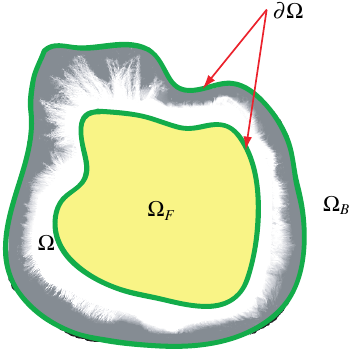
\includegraphics[width=3cm]{images/poissonRegion.png}
 \end{figure}
 \begin{itemize}
  \item User specifies known foreground $\Omega_F$ and known background
        $\Omega_B$.
  \item $(F-B)$ is initialized by differencing the spatially closest pixel
        in $\Omega_F$ and $\Omega_B$.
  \item Refining also consider pixels in $\Omega$ where $\alpha > 0.95$ for
        foreground and $\alpha < 0.05$ for background.
 \end{itemize}
\end{frame}

\begin{frame}[allowframebreaks]{Closed-Form Matting \cite{levin2008closed}}
 Poisson Matting used the input image to define the right-hand-side of the
 Laplace equation, but this work fixes the right-hand-side and uses the
 image to generate a data-dependent Laplace operator.
 \begin{itemize}
  \item The model depends on 2 assumptions:
  \begin{itemize}
   \item $\alpha = a_r I_R + a_g I_G + a_b I_B + a$ in a small window
   \item $F$ and $B$ are locally constant.
  \end{itemize}
  \item Supposedly, if $I$ is locally linear in color space, then $\alpha$
        can be written as that affine combination, but this is not clear.
 \end{itemize}
 \begin{figure}
  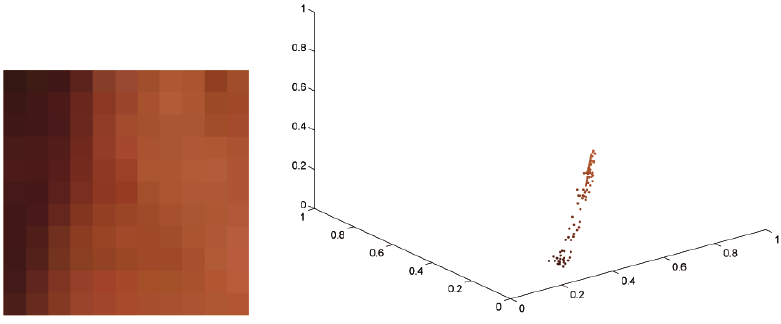
\includegraphics[width=4cm]{images/colorline.png}
 \end{figure}
 \begin{align}
  a_k(i,j) &\defeq 1 + (I_i-\mu_k)^T \left(\Sigma_k + \epsilon I\right)^{-1} (I_j-\mu_k) \\
  A_{ij} &\defeq \sum_{k \mid i,j \in w_k} \frac{1}{\lvert w_k \rvert} a_k(i,j) \\
  D_{ii} &\defeq \sum_j A_{ij} \\
  L &\defeq D-A
 \end{align}
 \begin{itemize}
  \item $a_k(i,j)$ is the similarity measure between pixels $i$ and $j$ in
        window $k$. $\mu_k$ is the mean pixel value in the window, and $\Sigma_k$
        is the $3 \times 3$ color covariance matrix in the window.
  \item $A_{ij} = A_{ji}$ is the ``global'' similarity between pixels $i$ and $j$.
  \item The idea is that $A_{ij}$ is large when $\alpha_i$ and $\alpha_j$ should be
        similar and small when they are unrelated.
  \item $D_{ii}$ is the degree of pixel $i$ under the similarity metric.
  \item $L$ is the Laplacian operator defined by the similarity measure.
  \item Now,
   \begin{align}
    \alpha^T L \alpha = \sum_{i~j} A_{ij}(\alpha_i-\alpha_j)^2
   \end{align}
   represents the amount that $\alpha$ deviates from the expectations we have
   under $A_{ij}$. In fact, this quadratic form defines an energy norm for $\alpha$.
  \item So, we want to solve
   \begin{align}
    \min_\alpha \; &\alpha^TL\alpha \\
    \text{s.t.} \; &\alpha_i = v_i \; \forall (i,v_i) \in \text{constraints} \nonumber \\
    \text{or} \nonumber \\
    (L + \gamma C) \alpha &= \gamma v,
   \end{align}
  \item $C$ is diagonal and $C_{ii}$ is 1 if $i$ is constrained.
  \item $\gamma$ is the Lagrange multiplier for the equality constraints.
  \item This has the same form as \eqref{eq:poisson}
 \end{itemize}
\end{frame}

\begin{frame}[allowframebreaks]{Learning-Based Matting \cite{zheng-learning}}
 Extends Closed-Form Matting by changing the pixel similarity metric.
 \begin{itemize}
  \item Like \cite{levin2008closed}, for a small window, we have the linear model
  \begin{align}
   \alpha_i =  I_i^T \beta + \beta_0
  \end{align}
  \item Stack the equations all $i$ in the window
  \begin{align}
   \alpha &=  I^T \beta + \beta_0, \; \text{or}\\
   \alpha &= \begin{bmatrix}I & 1\end{bmatrix} \begin{bmatrix} \beta \\ \beta_0 \end{bmatrix} \defeq X \begin{bmatrix} \beta \\ \beta_0 \end{bmatrix} \label{eq:alphacolor}
  \end{align}
  \item By least-squares regression,
  \begin{align}
   \begin{bmatrix} \beta \\ \beta_0 \end{bmatrix} = (X^TX+\lambda I)^{-1}X^T \alpha \label{eq:learning1}
  \end{align}
  \item So far, this is all a rehash of \cite{levin2008closed} with different notation.
  \item Notice in \eqref{eq:learning1} that $X^TX$ is $4 \times 4$ and
        represents inner products of window pixel values. I.e. $(X^TX)_{12}$
        is the inner product of the window's red channel with its green channel.
  \item They claim that \eqref{eq:learning1} can be rewritten as
  \begin{align}
   \begin{bmatrix} \beta \\ \beta_0 \end{bmatrix} = X^T(XX^T+\lambda I)^{-1} \alpha \label{eq:learning2}
  \end{align}
  \item Notice that \eqref{eq:learning1} is really the statement
        $\alpha = XX^+ \alpha$. This is true because (by assumption \eqref{eq:alphacolor}) $\alpha$
        is in the column space of $X$, and can therefore be recovered with the
        pseudoinverse.
  \item By the same reasoning, \eqref{eq:learning2} is the statement that
        $\alpha$ is \textit{also} in the column space of $XX^T$ and can be recovered by
        $\alpha = XX^T(XX^T)^+\alpha$.
  \item Notice that $XX^+$ has two eigenvalues, 0 and 1. Since $\alpha = XX^+ \alpha$,
        $\alpha$ must be a maximizer of $\alpha^T XX^+ \alpha$. This is the ``local''
        objective function and is summed over all windows to get the global objective
        function, which is still quadratic in $\alpha$.
  \item The matrix is $XX^T$, is $n \times n$ where $n$ is the number of
        pixels in the window, and whose entries are inner products of pixel colors.
  \item Suppose you have a feature extractor $\Phi(I)$
  \begin{align}
   \alpha = \Phi(I)^T \beta + \beta_0
  \end{align}
  \item By the kernel trick, there is a kernel $k(I_i,I_j) = \Phi(I_i)^T\Phi(I_j)$
  \item So, you can replace the colorspace inner products $XX^T$ with a matrix of
        kernel inner products.
  \item This paper uses the Gaussian kernel.
 \end{itemize}
\end{frame}

\begin{frame}[allowframebreaks]{Fast Matting \cite{he2010fast}}
 \begin{itemize}
  \item \cite{levin2008closed} is slow to solve, becuase $L$ is a very large
        sparse linear system with poor conditioning.
  \item It is useful to think about the Jacobi method when analyzing the speed.
        The Jacobi method solves independently for $\alpha^{k+1}_i$ for each
        element $i$ given $\alpha^k$ in the previous iteration $k$.
  \item Since the $i^\text{th}$ row of $L$ is nonzero only in a small $5 \times 5$
        radius, the value of $\alpha_i$ can only propagate to its $5 \times 5$
        neighborhood in 1 iteration.
  \item If the window size were bigger, the information would propagate more
        quickly, but $L$ would be less sparse (more work per iteration), and
        the quality will go down.
  \begin{figure}
   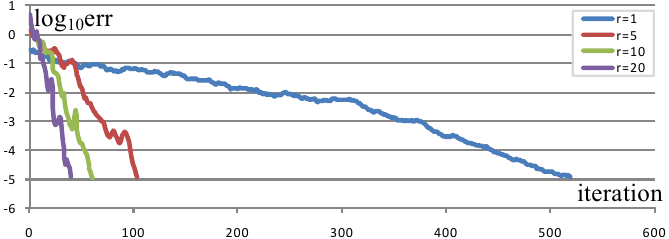
\includegraphics[width=6cm]{images/fastmatting_convergence.png}
   \caption{CG convergence with different window radius $r$}
  \end{figure}
  \item This work makes the time complexity of performing multiplication $Lp$ indepdendent of
        window size so that it is efficient to increase the window size to
        enhance convergence.
  \item To further speed it up, they propose breaking the image into segments
        that can be solved independently in parallel, then pieced together.
  \item The segments must each contain foreground and background constraints
        in order to be solved.
  \item The segmentation is done via KD tree, where the barycenter of the
        unknown region is computed, then a line passing through the point
        divides the region into two halves. This line is parallel to the
        $x$ or $y$ axis depending on if the unknown region is more spread
        out along those axes.
  \begin{figure}
   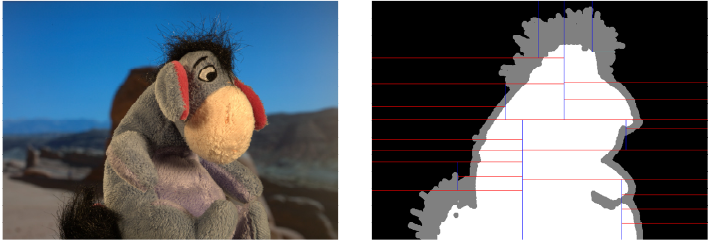
\includegraphics[width=8cm]{images/fastmatting_segmentation.png}
   \caption{Trimap segmentation.}
  \end{figure}
 \end{itemize}
\end{frame}

\begin{frame}[allowframebreaks]{Bayesian Matting \cite{chuang2001bayesian}}
 Builds Gaussian color models
 Does MAP estimation
 Propagates F and B
\end{frame}

\begin{frame}[allowframebreaks]{Grabcut \cite{rother2004grabcut}}
 Constructs color histograms using scribbles.
 Does hard segmentation by graph cut and color model.
 Fits polyline to boundary, and applies a smoothing function to get continuous $\alpha$
\end{frame}

\begin{frame}[allowframebreaks]{\cite{wang2005iterative}}
 Constructs local color models just as \cite{chuang2001bayesian}.
 Discretizes $\alpha$ to 25 levels.
 Uses belief propagation on uncertain nodes in an MRF to estimate unknown $\alpha$ values.
\end{frame}

\begin{frame}[allowframebreaks]{\cite{juan2005trimap}}
 Focuses not on matting, but the input to matting: trimaps and how to generate them.
 Uses color model and basic formulation of \cite{rother2004grabcut}.
 Defines a new model for blended F/G regions.
 Uses EM/MDL and Graph Cut for the trimap segmentation.
 Fast.
\end{frame}

\begin{frame}[allowframebreaks]{\cite{grady2005random}}
 The first Laplacian-based method?
 First solves a 3x3 colorspace eigenvalue problem to find a good linear
 color transformation that accentuates object boundaries.
 Defines graph adjacency with Gaussian kernel whose covariance matrix is
 the linear projector found above.
 Solves for the minimizer of $\alpha^TL\alpha$.
 GPU implementation.
\end{frame}

\begin{frame}[allowframebreaks]{Robust Matting \cite{wang2007optimized}}
 Focuses on generating the color models in \cite{chuang2001bayesian}.
 Uses different criteria to select points for modeling F and B distributions.
 Uses the formulation of \cite{levin2008closed} for Laplacian generation and solution.
 (Based on the 2006 version of that paper).
\end{frame}

\begin{frame}[allowframebreaks]{Geodesic Matting\cite{bai2007geodesic}}
 Builds color model
 Defines geodesic path distance based on color model
\end{frame}

\begin{frame}[allowframebreaks]{\cite{rhemann2008high}}
 Use Grab Cut \cite{rother2004grabcut} to generate trimap.
 Use Laplacian based on \cite{levin2008closed} and \cite{wang2007optimized}.
 They obtain a blurry matte, so they do deblurring based on the assumption that
 the true matte is binary.
\end{frame}

\begin{frame}[allowframebreaks]{Spectral Matting \cite{levin2008spectral}}
 Extends \cite{levin2008closed} a little.
 Mattes must be in the nullspace of Laplacian $L$, so extract a few of it's null vectors.
 Since the null vectors are not unique, want to find linear combinations that
 look like partial mattes.
 Solve a nonlinear problem involving the null vectors to produce ``matting components''
 that can be selected by user to give final matte.
\end{frame}

\begin{frame}[allowframebreaks]{\cite{duchenne2008segmentation}}
 Laplacian-based.
 Introduces spatial component to the colorspace Gaussian kernel of
 \cite{grady2005random} to define the Laplacian.
 Introduces scaling parameter $\lambda$ (equivalently $s$) to kernel.
 From what I can tell, this is just mostly explaining Laplacian methods. Not much novelty.
\end{frame}

\begin{frame}[allowframebreaks]{\cite{singaraju2009new}}
 Modifies color line assumption of \cite{levin2008closed}.
 In each local window, they inspect the rank of the color matrix.
 If it is less than 4, they use distinct local weightings based on line-point
 or point-point color models.
\end{frame}

\begin{frame}[allowframebreaks]{\cite{rhemann2010spatially}}
 Motivated by their previous work \cite{rhemann2008high}.
 Use \cite{rhemann2008high} to get initial matte.
 Upsample $\alpha$ by a factor of 3.
 Estimate binary matte at this scale with deconvolution, using assumption that
 the PSF is strongly peaked, but spatially varying.
 Use the PSF to blur the binary matte, then downsample to provide a prior on $\alpha$.
 Recover using the prior.
\end{frame}

\begin{frame}[allowframebreaks]{\cite{lee2011nonlocal}}
 Motivated by nonlocal denoising.
 Uses Laplacians.
 Instead of color similarity, use texture similarity to define graph weights.
 Construct nonlocal-based segmentation and allow user to select components
 to create trimap.
 Use variant of \cite{levin2008closed} to solve.
\end{frame}

\begin{frame}[allowframebreaks]{KNN Matting \cite{chen2012knn}}
 Improves \cite{lee2011nonlocal}.
 Uses FLANN to get the nonlocal neighbors (KNN).
 Uses $1-x$ kernel instead of exponential kernel.
\end{frame}

\begin{frame}[allowframebreaks]{\cite{chen2013image}}
 They just add a nonlocal smoothing term to the objective function.
 These assholes don't cite \cite{lee2011nonlocal}.
\end{frame}

\begin{frame}[allowframebreaks]{}
 
\end{frame}

% References ==================================================================
\begin{frame}[allowframebreaks]
 \frametitle{References}
 \bibliographystyle{amsalpha}
 \bibliography{mattingrefs.bib}
\end{frame}

\end{document}
